\noindent
%\section{Broadcast algorithm based on the diffusion model}
We now proceed to propose a broadcast algorithm based on the information diffusion model proposed earlier. 
Note that in contrast to the general assumption that size of a message is small enough to be transferred from one node to the other 
on the short duration of contacts between the nodes, we consider a more stringent case that is, the duration of a contact 
between the nodes is not always sufficient for the transfer and therefore the message might need to be 
segmented/divided into sub-parts and sent individually. Further note that our proposed diffusion model is a natural fit (which we elaborate next) as the 
number of contacts to contract infection can be replaced by the number of sub-parts in the message. 

%\vspace{-3.5mm}
\subsection{Agent configuration and network setup}
%\vspace{-2mm}
We consider a network topology $G = < V,E >$ where each node in $V$ represents an agent of the network and any link in $E$ represents a contact 
opportunity between a pair of nodes (agents) in the whole time span through which the network is active. So for any node (agent) $n_{i}$ in this network, its one hop 
neighbors are the nodes (agents) which are within the connection proximity of $n_{i}$ and at each time step $n_{i}$ at random can connect to any one of them. 


\subsection{Message configuration}
%\vspace{-2mm}
We consider that a message $\mathcal{M}$ is divided into a set of $m$ packets, i.e., $|\mathcal{M}| = m$. 
 Packets in $\mathcal{M}$ are grouped into a set $\mathcal{S}$ of $s$ segments, 
where each segment consists of $k = m/s$ packets (i.e., $s$ can take only those values for which $m \bmod s = 0$). 
For instance, if $\mathcal{M}$ constitutes of 4 packets and 2 segments then each of the segment is composed of 2 packets. 
%Note that we will mostly consider that there is only a single segment in the message ($m=k$) unless specified otherwise.

%\vspace{-5.9mm}
\subsection{Transfer protocol}
%\vspace{-2mm}
In this framework, transfer of a message during a contact refers to the transfer of one single packet of any segment of a message. 
Transfer of a packet from $u_i$ to $v_j$ during a contact can take place only 
when $u_i$ qualifies as a {\em sender} by having all the packets of at least one of the message segments. 
The two basic modes of message transfer that we consider are the push and the (restricted) pull epidemic. 

%\begin{itemize}
 %\vspace{-2mm}
 \noindent \emph{Push technique:} 
  \begin{itemize}
 % \vspace{-3mm}
   \item \emph{Step 1:} At any time step, $u_i$ (already a sender) establishes a communication link with $v_j$, 
   from its neighborhood and finds an exclusive set of packets that $u_i$ has but $v_j$ does not have in its buffer. 
   \item \emph{Step 2:} If $u_i$ can find such a (non-empty) set, then it transfers only one packet from this set to $v_j$. 
  \end{itemize}
  %Note that the \emph{push} technique is exactly similar to the diffusion model proposed earlier.
%\vspace{-2mm}
 \noindent \emph{Pull technique:} 
% \vspace{-3mm}
 \begin{itemize}
  \item \emph{Step 1:} At any time step, between $v_j$ and $u_i$, $v_j$ establishes a communication link with $u_i$ 
  and requests for a packet that it has not received yet. 
  \item \emph{Step 2:} Given that $u_i$ has already become a sender it first finds such a packet from its own buffer and then transfers a copy of it to $v_j$.
 \end{itemize}
  Note that in the traditional pull technique, $u_i$, being a sender, may transfer more than one packet if it gets multiple simultaneous requests from more than one agent at any particular time step. However, unlike the traditional case, here $u_i$ can serve only one request in case there are multiple pull requests. Such a restriction actually allows for conservation of both battery power and network bandwidth in resource constrained scenarios like DTN. 
  We further consider that the duration of each communication link is long enough for the transfer of at least a single packet.  


%\vspace{-5mm}
\subsection{Metrics of interest}
%\vspace{-2mm}
We are interested to evaluate the performance of a broadcast protocol in terms of two different metrics. The first metric concerns broadcast delay. 
The second metric centers around a complementary issue of power and bandwidth consumption.
\begin{itemize}
%\vspace{-4mm}
 \item \textbf{Broadcast delay $T^*$} - this is the time from the point when the message source starts sending the first packet to the point when all the agents in the network have received the entire message. 
 $E(T^*)$ denotes the expected broadcast time. 
 In addition, we are also interested in the time $t_i$ which is the minimum time at which there are $i$ senders (except the source) in the network, and especially in $t_1$ since, as we shall see, that this is the prime determinant of the entire broadcast time. 
 %\todo{why are these lines needed - Finally, note that $T^*$ may not correspond to $T_{n-1}$, i.e., the time when there are $n-1$ senders (except the source) in the network because all $n-1$ agents need not become senders to spread the message.}  
 \item \textbf{Broadcast wastage $C_m^*$} - let $C_l$ and $C_p$ be the total number of communication links that get established in the network and the total number of successful packet transfers respectively. We define the broadcast wastage as $C_m^* = (C_l - C_p)/C_l$. This metric essentially measures the number of useless contacts in the network during which no packet could be transferred and is therefore a direct cause of energy wastage.
\end{itemize}

\subsection{Broadcast algorithms}
We consider following four algorithms for broadcasting messages. While the first one (Blind Push) is exactly similar to the diffusion model proposed earlier, the others 
build on it.
\subsubsection{Blind push (B-P)}
{
An initiator node is the one which has the full message in the beginning. At each time step all the nodes 
in the system having the full message communicate with a node in their proximity and try to $push$. 
%If it is successful then a unit bandwidth is consumed otherwise it is counted as wastage. 
At the end of each time step all the nodes which have received all the packets qualify as sender in the next time step. The algorithm terminates 
when all the nodes in the system have the full message.}
% \vspace{-2mm}
% \begin{algorithm}[H]
%  %\KwData{this text}
%  %\KwResult{how to write algorithm with \LaTeX2e }
%  select initiator\;
%  make it sender\;
%  \While{not all nodes in the network have the message}{
%   \For{each node which is already a sender}{
%   select a node from its proximity;\\
%   perform $push$;\\
%   \eIf{$push$ unsuccessful}{
%   wastage;\\
%  }{unit bandwidth consumed;\\}
%  }
%  modify the list of senders;\\
%  increment time;\\
%  }
%  %\caption{Blind push (B-P) algorithm}
% \end{algorithm}
% \vspace{-4mm}
\subsubsection{Blind pull}
%The $Blind pull$ algorithm works the following way- Initially there is only a single node in the system which has the full message. 
At each time step 
all the nodes in the system not having the full message, communicate with a node in their proximity and try to $pull$. At the end of each time step 
the nodes which have received the full message stops pulling from the next time step. The algorithm terminates when all the nodes in the system have the full 
message.


\begin{figure}
\centering
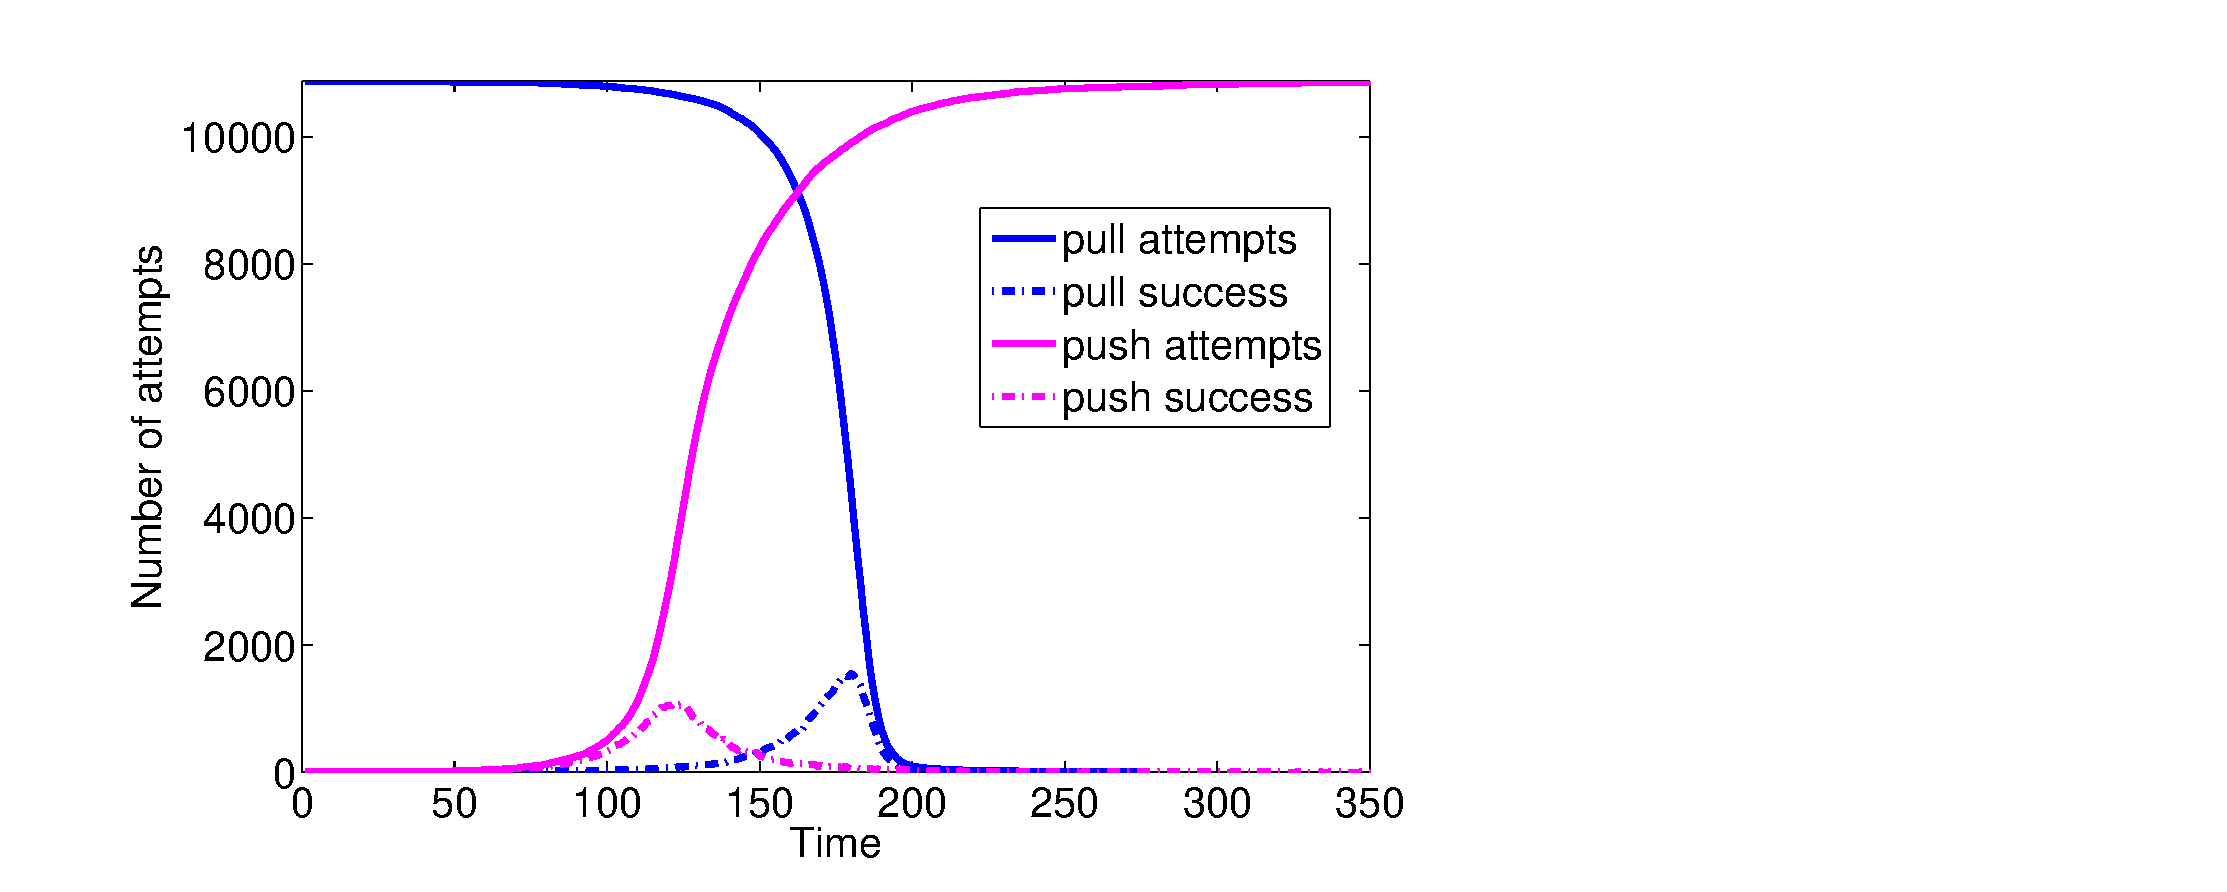
\includegraphics[scale=0.25]{./texfiles/Chapter_3/netsci/figs1/ps_pl_at_su.eps}
\caption{Pull attempts, successful pulls, push attempts, successful pushes versus time for gnutella1 network\vspace{4mm}}
\label{ps_pl_at_su}
\end{figure}

\subsubsection{Strategy-$x$\%, automatic switch from push to pull}

In this Strategy (X-P-P), the nodes in the system follow $Blind-push$ initially and then switch to $Blind-Pull$ once $x$\% of the nodes in the system have 
the full message. The algorithm terminates when all the nodes in the system have the full message.

We consider the $Blind-push$ and $Blind-pull$ algorithm on a network and check how efficiently they perform over a broadcast time window. 
In figure ~\ref{ps_pl_at_su} we plot the number of attempts and the number of successful ones for the above two cases on 
  gnutella1 network (described later in this section). 
  This clearly shows pull mechanism  
  performs poorly in the beginning but picks up after a certain percentage of nodes have become senders. We observe just the opposite behavior 
  for push mechanism. Our X-P-P strategy is based on this idea to obtain the best out of both the strategies.

The X-P-P strategy cannot be implemented in a practical setting  because every node in the system needs to maintain a global information of the percentage of nodes in the 
system having the full message which is difficult in a distributed setting like this.



\subsubsection{A distributed version of X-P-P strategy}
% To obtain a better coverage, we propose a combined strategy which combines $push$ and $pull$ in a practical way and is integrated with the give-up strategy to reduce wastage. We call this the 
% $Push Pull with giveup$ (P-P-G) technique.
% In this strategy,  each node $i$ maintains a counter ($pl\_count_i$, initialized to $0$) and an additional list $l_{i}$ which is initially empty.
% The counter counts
Here, we introduce a new strategy $Push-pull-with-giveup$ (P-P-G) which approximately mimics 
the X-P-P strategy in a distributed setting  and it functions in the following way - 
initially there  is a single node in the system which has the full message. At each time step the sender nodes in the system communicate with one of the nodes 
in their proximity and try to $push$. Among all the other non-sender nodes in the system those which have at least a single packet (i.e., nodes which have participated 
in a message transfer at least once and hence are aware of the broadcast) try to pull. Each node also keeps a local history regarding the number of unsuccessful 
communications it has participated in and once this exceeds a threshold, it `gives-up' and no longer 
participates in the broadcast. Once all the nodes have `given-up', the broadcast terminates.

% \begin{figure}
% \centering
% 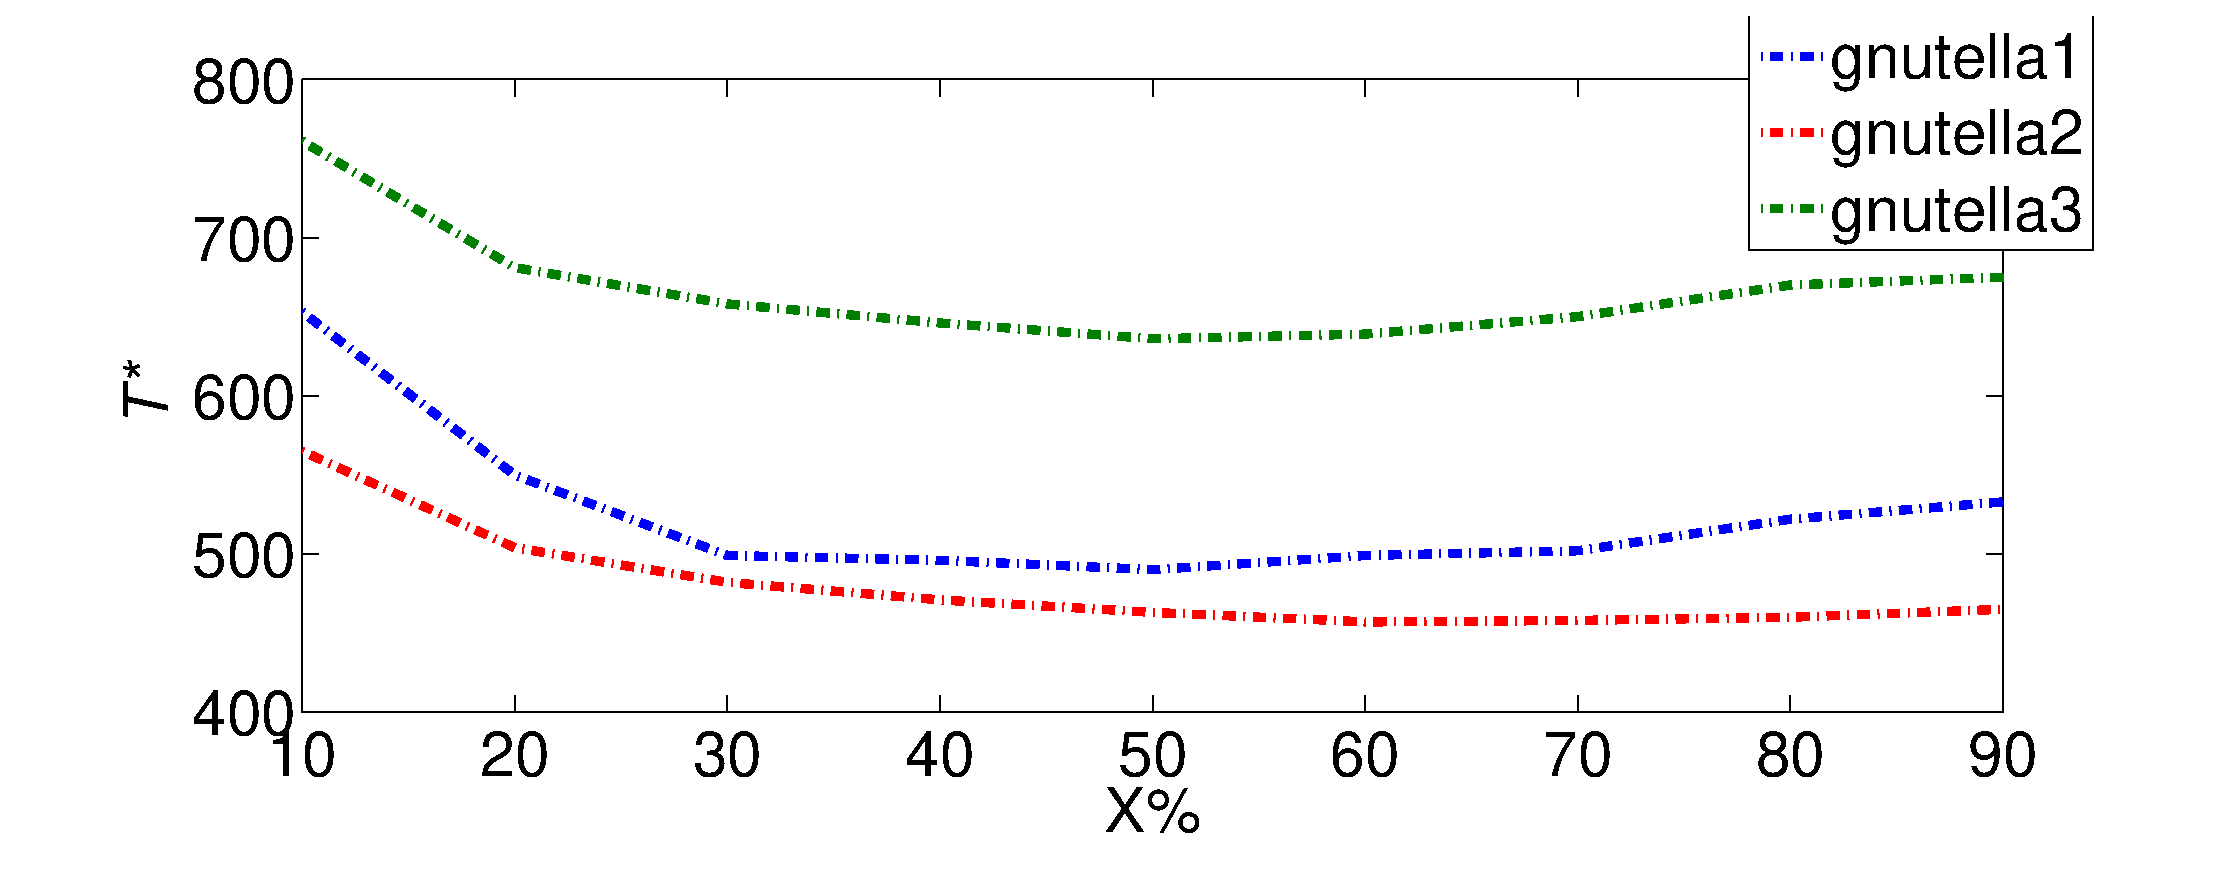
\includegraphics[scale=0.15]{figs1/xperbt.eps}
% 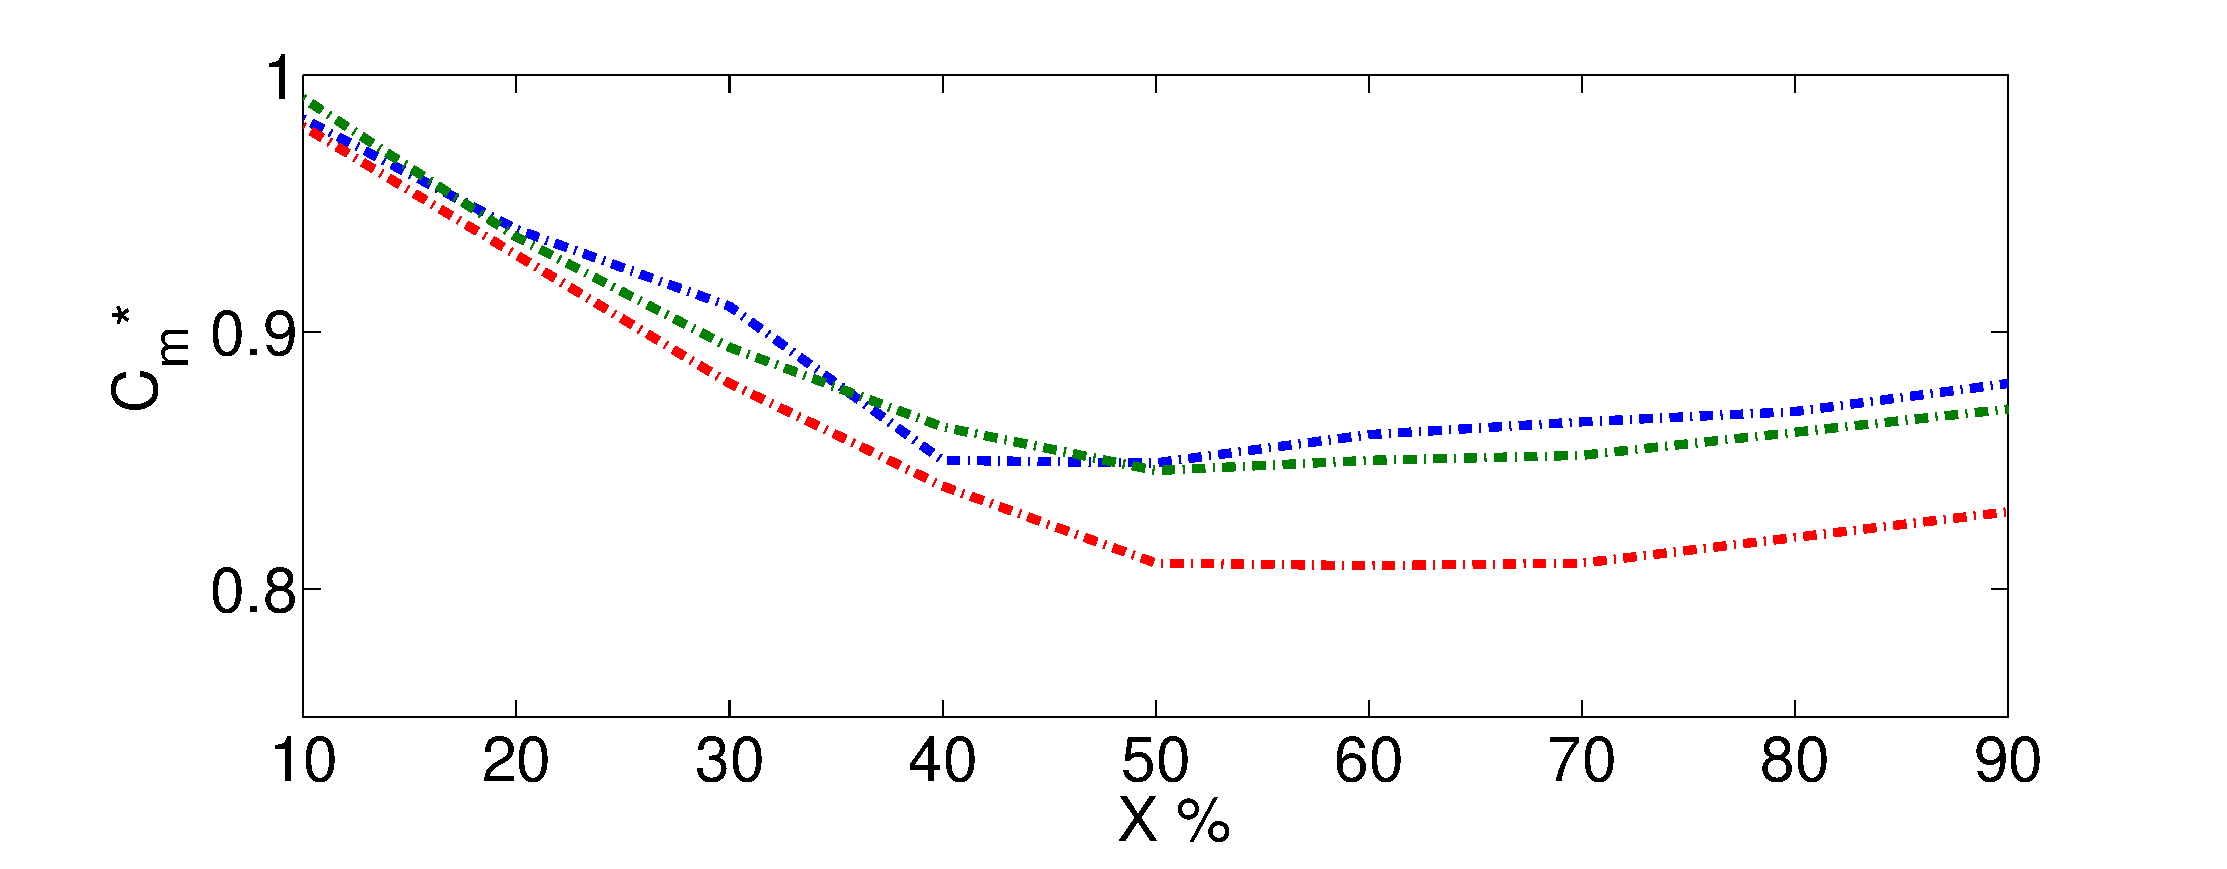
\includegraphics[scale=0.15]{figs1/xperwa.eps}
% \caption{Average broadcast time and wastage versus x for gnutella1,gnutella2 and gnutella3\vspace{-5mm}}
% \label{ps_bt}
% \end{figure}
% \medskip

\subsection{Dynamic topology}
%\vspace{-2mm}
We perform our experiments on gnutella snapshots and on synthetic topologies like complete graph, regular tree, regular graph and random graph. 
A topology specifies the potential neighborhood of a node 
- a node at each time step connects randomly to one of these nodes. A complete graph 
topology would indicate that the 
node can connect to any other node in the network while for other sparser topology it would 
connect only to a subset of them.
